%%%%%%%%%%%%%%%%%%%%
% Copyright and authorship of template: Fernando Oleo Blanco.
% Edited and expanded by : Nicolás Oriol Guerra
%
% Thanks to all the people that helped me get to where I am.
% Free use, just acknowledge the authors.
%%%%%%%%%%%%%%%%%%%%

\documentclass[12pt, a4paper]{article} % General document definition. In order to have the text completely centered, do not use the twoside option; however, twoside is recommended for printing.



%% PACKAGES

\usepackage[utf8]{inputenc} % Text encoding
\usepackage[english]{babel} % Choosing language
\usepackage{csquotes} % Needed for label

% Mathematical notation
\usepackage{amsmath, amsfonts, amssymb} 
 
 % TO make footnotes stay at the bottom of the page
 %\usepackage[bottom]{footmisc} 

% Section printing customization
\usepackage{titlesec} 

% To include pdf
\usepackage[final]{pdfpages} 

% To import images
\usepackage{graphicx} 
% https://www.overleaf.com/learn/latex/Inserting_Images


% To modify the geometry of pages (margins and other lengths)
\usepackage{geometry}

% To create tables
\usepackage{booktabs} 

% "Advance" and easier referencing
\usepackage{hyperref} 

% To add and format code
\usepackage{listings} 

% To have a wider array of colors available
\usepackage{xcolor} 

% Create a new command to highlight in red something
\newcommand\note[1]{\textcolor{red}{#1}} 
%\renewcommand\nota[1]{}} % Uncomment this to make all notes disappear

% Package for being able to "leave next page blank"  with the command % \afterpage{\blankpage}
\usepackage{afterpage} 
\newcommand\blankpage{%
    \null
    \thispagestyle{empty}%
    \addtocounter{page}{-1}%
    \newpage
    }
    
% Package for creating a box around the text. Needed for disclaimer page
\usepackage[linewidth=1pt]{mdframed}

% For setting linespaces when needed
\usepackage{setspace}

% To get some filler lorem ipsum text when needed
\usepackage{lipsum}

% Better centering format
\usepackage{ragged2e}


%\usepackage[backend=biber,style=numeric,citestyle=numeric,sorting=none]{biblatex}
\usepackage[hyperref,backend=biber,backref,backrefstyle=none, sorting = none, style = numeric]{biblatex}


%% Configuration

% Bibliography resource
\addbibresource{main.bib}

%\setlength{\parindent}{0pt}


%% DOCUMENT

\begin{document}
	
	

    	\begin{titlepage}
		\begin{figure}
			\centering
			\includegraphics[width=0.3\linewidth]{LogoUniversidadBN}
		\end{figure}
		\centering
		\Large Bachelor's Degree in Engineering in Telecommunication Technologies \\ 
		\vspace*{2em} % This just adds some vertical spacing
		\centering
		Bachelor's Final Project \\ 
		\vspace*{4em}
		Viability of PRIME Hybrid (PLC+RF) technology in low-voltage Smart Grid networks across different topologies.
        \\ \large
		\vspace*{6em}
		Author \\ Nicolás Oriol Guerra \\ 
		\vspace*{1em}
		Supervised by \\ Javier Matanza Domingo \\ Nicolás Arcauz Eguren % Supervisor(s) name(s) 
		% {\vfill \vspace*{3em}{Author's signature:\hrulefill \hfill} \hfill \\ \vspace*{4em}Supervisors' signatures:\hrulefill \hfill} % Uncomment this line if you would like to add a signature space
		\vfill
		Madrid  \\
		2021 -2022
	\end{titlepage}
	\blankpage
    
    \begin{mdframed}
    
 \begin{center}

\vspace*{2em}
I declare, under my responsibility, that the presented Project titled\\
\vspace*{1em}
{\large Viability of PRIME Hybrid (PLC+RF) technology in low-voltage Smart Grid networks across different topologies}\\
\vspace*{1em}
in the Engineering School - ICAI, Universidad Pontificia Comillas in the 2021/22 academic year is my own work, original and unpublished, and it has not been previously submitted for other purposes.\\
\vspace*{1em}
This project is not plagiarism of any other work, neither totally nor partially and all contributions by other authors have been dully referenced.

\vspace*{3em}
Declaro, bajo mi responsabilidad, que el Proyecto presentado con el título\\
\vspace*{1em}
{\large Viabilidad de la tecnología PRIME Híbrida (PLC + RF) para distintas topologías de redes inteligentes de baja tensión}\\
\vspace*{1em}
en la ETS de Ingeniería - ICAI de la Universidad Pontificia Comillas en el curso académico 2021/22 es de mi autoría, original e inédito y no ha sido presentado con anterioridad a otros efectos. \\
\vspace*{1em}
El Proyecto no es plagio de otro, ni total ni parcialmente y la información que ha sido tomada de otros documentos está debidamente referenciada.\\

\vspace*{3em}
Nicolás Oriol Guerra \hspace{2.6cm}  Date:

\vspace*{2em}
Project's delivery authorized\\
Autorizada la entrega del proyecto\\

\vspace*{1em}
THE PROJECT'S SUPERVISOR\\
EL DIRECTOR DEL PROYECTO\\


\vspace*{2em}
Javier Matanza Domingo \hspace{2cm}  Date:\\

\vspace*{3em}

\end{center}    
    
\end{mdframed}

    
    % Lío enorme pero funciona
    \thispagestyle{empty} % Do not show page numbering
    \newpage
    \thispagestyle{empty}%
    \blankpage
    
    
    	\begin{titlepage}
		\begin{figure}
			\centering
			\includegraphics[width=0.3\linewidth]{LogoUniversidadBN}
		\end{figure}
		\centering
		\Large Bachelor's Degree in Engineering in Telecommunication Technologies \\ 
		\vspace*{2em} % This just adds some vertical spacing
		\centering
		Bachelor's Final Project \\ 
		\vspace*{4em}
		Viability of PRIME Hybrid (PLC+RF) technology in low-voltage Smart Grid networks across different topologies.
        \\ \large
		\vspace*{6em}
		Author \\ Nicolás Oriol Guerra \\ 
		\vspace*{1em}
		Supervised by \\ Javier Matanza Domingo \\ Nicolás Arcauz Eguren % Supervisor(s) name(s) 
		% {\vfill \vspace*{3em}{Author's signature:\hrulefill \hfill} \hfill \\ \vspace*{4em}Supervisors' signatures:\hrulefill \hfill} % Uncomment this line if you would like to add a signature space
		\vfill
		Madrid  \\
		2021 -2022
	\end{titlepage}
    \blankpage
    
    \pagenumbering{roman}
    \setcounter{page}{1}
    
    \noindent
\centerline{{\large Viability of PRIME Hybrid (PLC+RF) technology}} 
\centerline{{\large in low-voltage Smart Grid networks across different topologies}}\\

\noindent
\centerline{{\small Author: Oriol Guerra, Nicolás}}
\centerline{{\small Supervisors: Matanza Domingo, Javier; Argauz Eguren, Nicolás}}
\centerline{{\small Collaborating Entity: Iberdrola}}

\subsection*{Abstract}
\subsection*{1. Introduction}
Lorem ipsum dolor sit amet, consectetur adipisicing elit, sed do eiusmod tempor incididunt ut labore et dolore magna aliqua. Ut enim ad minim veniam, quis nostrud exercitation ullamco laboris nisi ut aliquip ex ea commodo consequat. 
Lorem ipsum dolor sit amet, consectetur adipisicing elit, sed do eiusmod tempor incididunt ut labore et dolore magna aliqua. Ut enim ad minim veniam, quis nostrud exercitation ullamco laboris nisi ut aliquip ex ea commodo consequat\\

\textbf{Keywords}: keywordA, keywordB, keywordC

\subsection*{2. Objective definition}
Lorem ipsum dolor sit amet, consectetur adipisicing elit, sed do eiusmod tempor incididunt ut labore et dolore magna aliqua. Ut enim ad minim veniam, quis nostrud exercitation ullamco laboris nisi ut aliquip ex ea commodo consequat. 
Lorem ipsum dolor sit amet, consectetur adipisicing elit, sed do eiusmod tempor incididunt ut labore et dolore magna aliqua. Ut enim ad minim veniam, quis nostrud exercitation ullamco laboris nisi ut aliquip ex ea commodo consequat

\subsection*{3. Description of simulation model}
Lorem ipsum dolor sit amet, consectetur adipisicing elit, sed do eiusmod tempor incididunt ut labore et dolore magna aliqua. Ut enim ad minim veniam, quis nostrud exercitation ullamco laboris nisi ut aliquip ex ea commodo consequat. 
Lorem ipsum dolor sit amet, consectetur adipisicing elit, sed do eiusmod tempor incididunt ut labore et dolore magna aliqua. Ut enim ad minim veniam, quis nostrud exercitation ullamco laboris nisi ut aliquip ex ea commodo consequat

\subsection*{4. Results}
Lorem ipsum dolor sit amet, consectetur adipisicing elit, sed do eiusmod tempor incididunt ut labore et dolore magna aliqua. Ut enim ad minim veniam, quis nostrud exercitation ullamco laboris nisi ut aliquip ex ea commodo consequat. 
Lorem ipsum dolor sit amet, consectetur adipisicing elit, sed do eiusmod tempor incididunt ut labore et dolore magna aliqua. Ut enim ad minim veniam, quis nostrud exercitation ullamco laboris nisi ut aliquip ex ea commodo consequat

\subsection*{5. Conclusions}
Lorem ipsum dolor sit amet, consectetur adipisicing elit, sed do eiusmod tempor incididunt ut labore et dolore magna aliqua. Ut enim ad minim veniam, quis nostrud exercitation ullamco laboris nisi ut aliquip ex ea commodo consequat. 
Lorem ipsum dolor sit amet, consectetur adipisicing elit, sed do eiusmod tempor incididunt ut labore et dolore magna aliqua. Ut enim ad minim veniam, quis nostrud exercitation ullamco laboris nisi ut aliquip ex ea commodo consequat

    \newpage
    
    \noindent
\centerline{{\large Viabilidad de la tecnología PRIME Híbrida (PLC + RF)}} 
\centerline{{\large para distintas topologías de redes inteligentes de baja tensión}}\\

\noindent
\centerline{{\small Autor: Oriol Guerra, Nicolás}}
\centerline{{\small Director: Matanza Domingo, Javier; Argauz Eguren, Nicolás}}
\centerline{{\small Entidad Colaboradora: Iberdrola}}

\subsection*{Resumen}
\subsection*{1. Introducción}
Lorem ipsum dolor sit amet, consectetur adipisicing elit, sed do eiusmod tempor incididunt ut labore et dolore magna aliqua. Ut enim ad minim veniam, quis nostrud exercitation ullamco laboris nisi ut aliquip ex ea commodo consequat. 
Lorem ipsum dolor sit amet, consectetur adipisicing elit, sed do eiusmod tempor incididunt ut labore et dolore magna aliqua. Ut enim ad minim veniam, quis nostrud exercitation ullamco laboris nisi ut aliquip ex ea commodo consequat\\

\textbf{Palabras clave}: keywordA, keywordB, keywordC

\subsection*{2. Definición de objetivos}
Lorem ipsum dolor sit amet, consectetur adipisicing elit, sed do eiusmod tempor incididunt ut labore et dolore magna aliqua. Ut enim ad minim veniam, quis nostrud exercitation ullamco laboris nisi ut aliquip ex ea commodo consequat. 
Lorem ipsum dolor sit amet, consectetur adipisicing elit, sed do eiusmod tempor incididunt ut labore et dolore magna aliqua. Ut enim ad minim veniam, quis nostrud exercitation ullamco laboris nisi ut aliquip ex ea commodo consequat

\subsection*{3. Descripción del modelo de simulación}
Lorem ipsum dolor sit amet, consectetur adipisicing elit, sed do eiusmod tempor incididunt ut labore et dolore magna aliqua. Ut enim ad minim veniam, quis nostrud exercitation ullamco laboris nisi ut aliquip ex ea commodo consequat. 
Lorem ipsum dolor sit amet, consectetur adipisicing elit, sed do eiusmod tempor incididunt ut labore et dolore magna aliqua. Ut enim ad minim veniam, quis nostrud exercitation ullamco laboris nisi ut aliquip ex ea commodo consequat

\subsection*{4. Resultados}
Lorem ipsum dolor sit amet, consectetur adipisicing elit, sed do eiusmod tempor incididunt ut labore et dolore magna aliqua. Ut enim ad minim veniam, quis nostrud exercitation ullamco laboris nisi ut aliquip ex ea commodo consequat. 
Lorem ipsum dolor sit amet, consectetur adipisicing elit, sed do eiusmod tempor incididunt ut labore et dolore magna aliqua. Ut enim ad minim veniam, quis nostrud exercitation ullamco laboris nisi ut aliquip ex ea commodo consequat

\subsection*{5. Conclusiones}
Lorem ipsum dolor sit amet, consectetur adipisicing elit, sed do eiusmod tempor incididunt ut labore et dolore magna aliqua. Ut enim ad minim veniam, quis nostrud exercitation ullamco laboris nisi ut aliquip ex ea commodo consequat. 
Lorem ipsum dolor sit amet, consectetur adipisicing elit, sed do eiusmod tempor incididunt ut labore et dolore magna aliqua. Ut enim ad minim veniam, quis nostrud exercitation ullamco laboris nisi ut aliquip ex ea commodo consequat

    \newpage
    
    \tableofcontents
    \newpage
    
    \listoffigures
    \newpage
    
    \listoftables
    \cleardoublepage
    
    \pagenumbering{arabic}
    \setcounter{page}{1}
    
    \section{Introduction}
\subsection{The electrical grid's current trajectory}
The electrical grid is a system composed of many interconnected pieces. Each of these pieces interacts with the others and contributes to achieving the network's ultimate goal: managing energy supply and demand to accommodate individual demand schedules with centralized and distributed generation. This system is highly complex, and its three main stages - generation, transmission, and distribution - are continuously evolving.

The electrical system has a global presence. However, it cannot be envisioned as one homogeneous unit, rather as a set of interconnected networks. Even though they have different characteristics (topologies, physical magnitudes, standards) there are some challenges and threats that are common to all networks. 


As described in \cite{the_new_frontier_of_smart_grids}, these challenges include planning inefficiencies, periodic consumption patterns with high peak-valley differences, and congestion and loss in transmission and distribution. Most of these boil down to the one factor that distinguishes electrical energy from other commodities: electricity cannot be stored efficiently in large quantities, thus supply must equal demand at all times. From this fact, several problems arise which require that the whole system be resilient and managed with low latencies. Resilience is key because any failure in the system has immediate consequences that can be felt at other points in the network. Low latency allows decisions to be made with up-to-date information, facilitates fault correction, and improves automation capabilities \cite{telco_ntwks_for_the_smart_grid}.

These problems are not new to the industry. However, the scale at which they are now occurring and other factors, such as the increasing share of renewable energy generation,  require the incorporation of new solutions. The set of new solutions and improvements designed to improve the network - which are mainly based on telecommunication services - is nowadays known as the \textit{Smart Grid}. 


\subsection{Low-voltage distribution networks}\label{section_introduction_subsection_lv_networks}
Special attention will be dedicated to de distribution stage of the electrical network. Particularly, low-voltage (LV) distribution networks. This part of the network consists of lines with voltage levels below 1kV. They are the most diverse part of the network as its topology highly depends on the individual population and service area \cite{telco_ntwks_for_the_smart_grid}. For now, it is important to state that MV/LV transformers\footnote{Device that reduces voltage to adequate levels for distribution amongst households, small businesses and medium-sized industrial customers} are part of the distribution networks and are feeding LV lines, connecting them to the MV grid. Thus, given the network's topology, secondary substations are placed in a prime location to boost MV and LV digitization. 

Key Smart Grid applications at LV distribution include Demand Response (DR) and Automatic Meter Management (AMM). Both of these features make use of bidirectional communications between utilities and consumers. DR uses these interactions to facilitate more efficient generation and consumption patterns. AMR allows utilities to collect information automatically from consumers by communicating with electricity meters.

This communication can be done with different technologies such as powerline communication (PLC) or wireless radio-frequency communications (RF). PLC is currently one of the most widespread communication technologies for LV networks. PLC's biggest advantage is that information travels through an already established medium. This channel is pre-existing powerlines, which means that no additional infrastructure rollout is required \cite{primeWhitePaper}.  However, it is not the best technology for all scenarios due to the possibility of noisy channels, non-dense populations and non-existing or unsuitable electric rollouts. In such scenarios, RF communication may be the superior technology. A few reasons why RF may be more suitable in some instances are emission regulations, and high variability of attenuation depending on the communication scenario. High regulations ensure that communications take place in a controlled noise environment whereas a high range of possible attenuation means that RF will be suitable in at least some scenarios.


\subsection{Focus of the study}\label{section_introduction_subsection_focus_of_the_study}
It is at this point where this study will focus. Both technologies have provided positive results independently \cite{prime_hybrid_solution_combines_plc_and_rf}. However, they both have their weaknesses. The merging of both of them in a hybrid solution provides a more flexible and reliable network. PRIME Alliance\footnote{PoweRline Intelligent Metering Evolution} has merged them into a hybrid standard solution: PRIME Hybrid.

We will delve deeper into this standard set by PRIME Alliance in section \ref{section_state_of_the_art}. For now, it can be established that this paper aims to study the viability of the PRIME Hybrid solution for different LV network topologies. To achieve this, a simulation framework based on the PRIME simulator described in \cite{tesis_jmatanza} will be developed. The simulator will be expanded to include the newest version of PRIME specifications and RF capabilities. Finally, an economic comparison will be done with other rollout alternatives (such as the Wi-SUN alliance and/or LTE).

The expected results are a comprehensive comparison of PRIME Hybrid performance across different scenarios and a high-level analysis of the cost-benefit structure of the different rollout alternatives.
    \cleardoublepage
    
    \section{State of the art}\label{section_state_of_the_art}

The academic field concerning Smart Grids and their applications has seen a substantial rise in popularity in recent years. It is certainly relevant to base the present paper on available conclusions and published work. This section is organized as follows. First, some background is provided on PRIME Alliance in section \ref{section_state_of_the_art_subsection_PRIME_Alliance}. Then, PLC and RF standards are discussed separately in sections \ref{section_state_of_the_art_subsection_PRIME_13_14} and \ref{section_state_of_the_art_subsection_802}. The combination of both standards is discussed in section \ref{section_state_of_the art_subsection_prime_hybrid}.


\subsection{PRIME Alliance}\label{section_state_of_the_art_subsection_PRIME_Alliance}
PRIME Alliance (PoweRline Intelligent Metering Evolution) is a worldwide organization whose main goal is to support smart metering and smart grid functionalities. They strive to pursue this by developing and maintaining standardized telecommunication solutions which are publicly available. It was created in 2009 and up until today, solutions with PRIME standards have been applied globally (Spain\footnote{In Spain, PRIME solution represents the most widely adopted standard}, Portugal, Poland, Brasil...) with high levels of success \cite{prime_alliance_description_document}. Discussion regarding this organization is relevant because the PLC standard and hybrid solution used in the simulation are based on published PRIME Alliance information.

\subsection{PRIME v1.3 and v1.4}\label{section_state_of_the_art_subsection_PRIME_13_14}
PRIME is a powerline communication (PLC) standard with presence throughout the globe. It is based on OFDM (orthogonal frequency division multiplexing) technology and it can operate in MV and LV networks. It was developed for "Advanced Metering, Grid Control and Asset Monitoring applications". One of its key benefits is the achieved interoperability between different manufacturers which has resulted in more than 20 million smart meters deployed worldwide \cite{prime_alliance_description_document}.

The standard, has been recently updated to PRIME v1.4. This update was undertaken in 2014 \cite{prime_v14_evolution_a_future__proof_of_reality_beyond_metering} and adds additional robustness options and extended frequency coverage (up to 500kHz from the prior 90kHz) to the previous version PRIME v1.3.

The PRIME standard defines two kinds of network nodes: Base Node (BN) and Service Node (SN). The base node manages the network and coordinates the responses from a pool of service nodes. This BN is usually located in the MV/LV transformer (see section \ref{section_introduction_subsection_lv_networks}). A network is comprised of multiple SN registered to one BN. Thus, the network is managed by a BN which periodically polls SN to obtain updated information of all devices connected to the network.

Previous works related to the topic at hand include the following. In \cite{tesis_jmatanza}, the author discusses several PLC standards and develops a simulated environment to test them. In \cite{prime_v14_evolution_a_future__proof_of_reality_beyond_metering}, the authors discuss the uses of PRIME v1.4 and provide an overview of the improvements of the new version. Other important documents that will be taken into account are the white papers distributed by PRIME Alliance \cite{primeWhitePaper}, and the standard specifications \cite{prime_v14_specifications}.


\subsection{Wireless RF, standard 802.15.4}\label{section_state_of_the_art_subsection_802}
IEEE 802.15.4 is a standard developed for low-rate wireless networks. It was first devised in 2003 and it has been updated continuously over the years with its latest revision being in 2020. The goal of this standard since its inception was the creation of inexpensive, low-power communications.

802.15.4 defines a physical layer (PHY) and a medium access control layer (MAC). It describes two types of devices that can participate in the network: full-function devices (FFD) and reduced-function devices (RFD). The difference between them is that a FFD is able to participate in the network serving as a personal area network (PAN) coordinator. On the other hand, RFD are intended to serve only for simple applications. One FFD is assigned to multiple RFD at a time, however the inverse is not true. One RDF can only have one FFD assigned at one time. Thus, the FFD plays the part of the network coordinator described in the PRIME standard.

Several papers such as \cite{theoretical_analysis_of_report_success_probability_in_IEE_802154} and \cite{experimental_perf_evaluation_802154_SUN} have performed analysis regarding the implementation of this standard in smart utility networks (SUN). The combination of this with PLC communications is discussed in the following section.



\subsection{PRIME Hybrid}\label{section_state_of_the art_subsection_prime_hybrid}
The combination of both PLC and RF technologies is the latest tendency promoted by PRIME Alliance. The expected benefits of this combination have been laid out in previous sections (see section \ref{section_introduction_subsection_focus_of_the_study}) and are a key focus of the current study. 

The basis of this hybrid solution is the addition of RF specifications into the PRIME v1.4 stack of protocols. This will allow nodes to communicate amongst each other whether they are PLC-only, RF-only or hybrid nodes containing both technologies. 

The combination of both specifications is achieved by integrating both PHY layers onto the same MAC layer (defined by PRIME v1.4). This allows for a fully backward-compatible solution that will include the best of both alternatives.

The hybrid alternative is a relatively new idea. It has been proposed and discussed in several papers such as \cite{prime_hybrid_solution_combines_plc_and_rf, evolution_of_prime_to_plc_rf_hybrid_systems, toward_more_efficient_more_secure_PLC_RF_Hybrid}. Most of these papers stay at a theoretical level when discussing the hybrid approach. A well-documented example of a simulation and implementation of the technology is \cite{toward_more_efficient_more_secure_PLC_RF_Hybrid}. In this paper, the author sets up an outdoor experiment with street lamps controlled via PLC or RF. However, the proposed method does not allow a node to switch between the two technologies when needed. Instead, lamps are randomly assigned a transmission method (PLC or RF) and the experiment is run for that network configuration. Furthermore, the topology of the network and the number of connected nodes stays constant throughout the experiment. These two characteristics are results that this study aims to alter and consider. By taking into account both of these parameters, obtained results will have interesting implications for network deployment and planning.






 


    \cleardoublepage
    
    %% OK con Grammarly

\section{Motivation}

\subsection{Metering evolution in the Spanish market}
In December 2007, the Spanish government approved the required legislation \cite{boe_renovacion_contadores_2007} "by which all electrical invoices from January 2008 onward must be modernized". In this document, the Government imposes on utility companies the duty to replace all qualifying electricity meters. The measuring equipment would qualify for replacement if contracted power was lower than 15kW\footnote{Average contracted power for a Spanish household is 4kW with an average monthly consumption of 270kWh \cite{ree_consumo_medio}}.

The reason behind this metering overhaul was to install more up-to-date electricity meters. These meters would have hourly discrimination and remote management capabilities. The legislation was updated again in 2012 \cite{boe_renovacion_contadores_2012} to revisit the intermediate milestones while maintaining the final deadline. The final schedule and milestones were: substituting 35\% of meters before 2015; another 35\% before 2017; and the final 30\% before 2019.

According to a report published by \textit{Comisión Nacional de los Mercados y la Competencia (CNMC)}\footnote{Spanish equivalent of European Securities and Markets Authority (ESMA)} the outcome of this metering renovation initiative was a success. By December 31st 2018, 99.04\% of new meters had already been installed \cite{cnmc_renovacion_contadores}. This modernization brought several new crucial tools to the table. The most prominent ones are the automatic readings of users' electric consumption, and more flexible tariff offers (for example with hourly price discrimination).

Nowadays, energy companies are faced with new challenges to improve the overall performance of the electrical grid and increase their operating efficiency. Players must keep updating and renewing their equipment to achieve higher network efficiency and operating flexibility. The final goal is to have a grid with bidirectional communication, automated operations control, and the ability to efficiently collect information generated by consumers and distributed generation units connected to the network. To face these upcoming challenges, the Spanish Government has kept-up legislative pressure to innovate. Electric meters must be renewed again before February 2025 \cite{boe_renovacion_contadores_2020}.

\subsection{Scope of the study within the metering evolution}
At this point is where the present study comes into play. Energy utilities are currently considering different network improvement options. One of these alternatives is the introduction of PRIME Hybrid technology as a means of communicating with end-user meters. In addition to studying the case of the Spanish grid - where PLC communications have already been successfully introduced - PRIME Hybrid will also be tested for other geographies.

Network topologies for Brazil and the United States will be simulated. These countries have fundamentally different characteristics to those of the Spanish electrical system.  For example, where PLC installation is concerned, Spain was an attractive network for this kind of rollout. Spain's fit with PLC technology is mainly due to the high client to substation ratio (around 100 clients per substation)\footnote{A higher number of supply points per substation significantly reduces the scale of the required rollout and its total cost. In this context, substation is referring to MV/LV transformers which are sometimes called \textit{secondary} substations}. Higher ratios imply less capital expenditures per household when deploying the technology which decreases the overall cost of updating the whole grid. This ratio is lower in both the US, and Brazil (the former with around 2 clients per substation and the latter sitting in between the US and Spain) \cite{conversacion_nico_arcauz}. In these cases, RF may provide a  more viable alternative to PLC due to potentially easier installations, higher ranges and lower costs. A combination of the two technologies (PRIME Hybrid) may be the most suitable choice. This is the starting point for our analysis and the motivation to create a simulation tool with capabilities to obtain results comparing RF, PLC and the combination of the two in PRIME Hybrid. These comparisons will be established across different network scenarios and topologies.
    \cleardoublepage
    
    \section{Objectives}

This project has three main objectives. The PRIME Hybrid simulation tool will be developed to reach meaningful conclusions in all three goals.

\begin{itemize}
  \item Consider the viability of a PRIME Hybrid solution (PLC + RF).
  \item Understand the possible discrepancies and gray areas that arise when combining PLC and RF standards. A potential approach to these unclear points will be proposed.
  \item Examine the effectiveness of a PRIME Hybrid solution by simulating a network under different working conditions.
\end{itemize}

The development of the simulation tool is not an objective in itself. It will be crucial in reaching the objectives listed above but it will be considered as a means to an end, a tool used to reach the main conclusions. Further explanation is provided below regarding how to achieve the proposed goals.


\begin{description}
    \item \textbf{Viability of Hybrid solution.} Before diving fully into the development of the simulation tool, an analysis will be done regarding the compatibility of the different standards. The possibility of combining the protocol stacks of PLC and RF needs to be studied and understood. To achieve this, an explanation is provided regarding the newest PRIME standard (v1.4) and how to include an RF PHY layer in its protocol stack.
    \item \textbf{Gray areas in standards.} The merging of PLC and RF is expected to not be seamless. Any decisions taken in the process that are not fully detailed in current standards will be laid out and discussed. For example, if the node's choice to use PLC or RF is dynamic, several possible decision parameters will be considered.
    \item \textbf{Effectiveness of Hybrid solution.} Simulations will help measure the results of hybrid communications and how they compare to PLC and RF individually. Some expected results are network latencies, throughput and availability. 
\end{description}

    \cleardoublepage
    
    %% OK con Grammarly

\section{Methodology}
The project's methodology is detailed in two steps. First, the project's action plan is laid out and explained. Then, a timeline is presented with the work distribution and weekly milestones.

\subsection{Project phases}

The proposed analysis will be structured into five phases shown in Figure \ref{fig:plan_accion}. In this section, the work to be performed is defined in each of the five steps. Section \ref{cronograma} provides finer details regarding the timeline of each step.


\begin{figure}[h!]
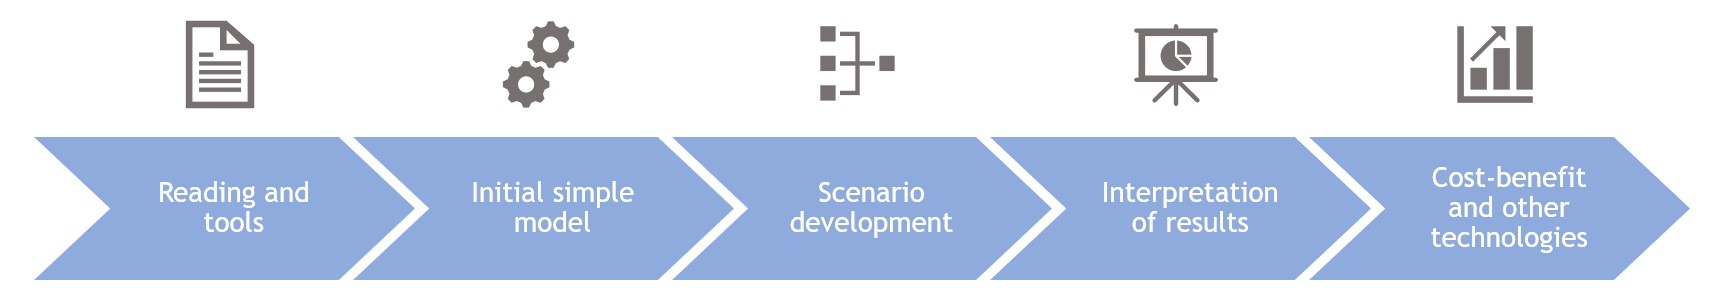
\includegraphics[width=\textwidth]{images/metodologia_trabajo_1.jpg}
\caption{Proposed action plan}
\label{fig:plan_accion}
\centering
\end{figure}


\begin{description}
   \item[Reading and tools.] Read PRIME 1.4 and standard 802.15.4 documentation. Investigation and documentation regarding the state of the art and related topics. Preparation of the OMNeT environment \cite{omnet} and the SimPRIME library \cite{simprime}. Understand the simulation tools, simulate simple scenarios, and ensure legacy code is working as intended.
   \item[Initial simple model.] Independent scenario testing of PRIME and RF technologies. Analyze the results separately and ensure they are in line with expected theoretical outcomes. After this has been achieved, join both scenarios to create a simple model where both technologies work as intended.
   \item[Scenario development.] Define which parameters to compare in the study. Once they have been defined, we will generalize and tweak the previous code to collect results according to the chosen parameter values (these values are defined in the following phase). The final goal of this step is to have a functional PRIME Hybrid simulation with the ability to introduce variable entry parameters.
   \item[Interpretation of results.] Gather all relevant information and characteristics of scenarios to simulate. With this information, parameter values will be defined to run the simulations. Their outcome will be analyzed.
    \item[Cost-benefit and other technologies.] The conclusions reached from comparing the various scenarios will be compared with high-level results from other technologies. In this step, a cost-benefit analysis will also be performed to further compare PRIME Hybrid with alternative network communication technologies.
\end{description}



\subsection{Timeline}\label{cronograma}

The project has an estimated duration of 34 weeks. The starting date is October 11th 2021. The project will end on the week of May 30th 2022 with the final project presentation. A Gantt diagram with the detailed timeline is presented at the end of the document.


    \cleardoublepage
    
    % Ok con Grammarly

\section{Resources}

This project will mainly make use of the OMNeT \cite{omnet} simulation tool. This program is a discrete event simulator based on modules described in C++. OMNeT allows for network modeling by independently defining each of the components - with their respective protocol stacks - and channels. In \cite{prime_replicability} the author shows an example of modeling PRIME technology with this tool. The main libraries used will be INET \cite{inet} and SimPRIME \cite{simprime}.

Matlab will be used to simulate the physical layer (PHY) and to obtain the characteristics of each communication channel. This method is similar to the one proposed in \cite{tesis_jmatanza}. To analyze the final results and plot graphics \textit{plotly} - an open-source Python library - will be used.

    \cleardoublepage
	
	\printbibliography
	
	%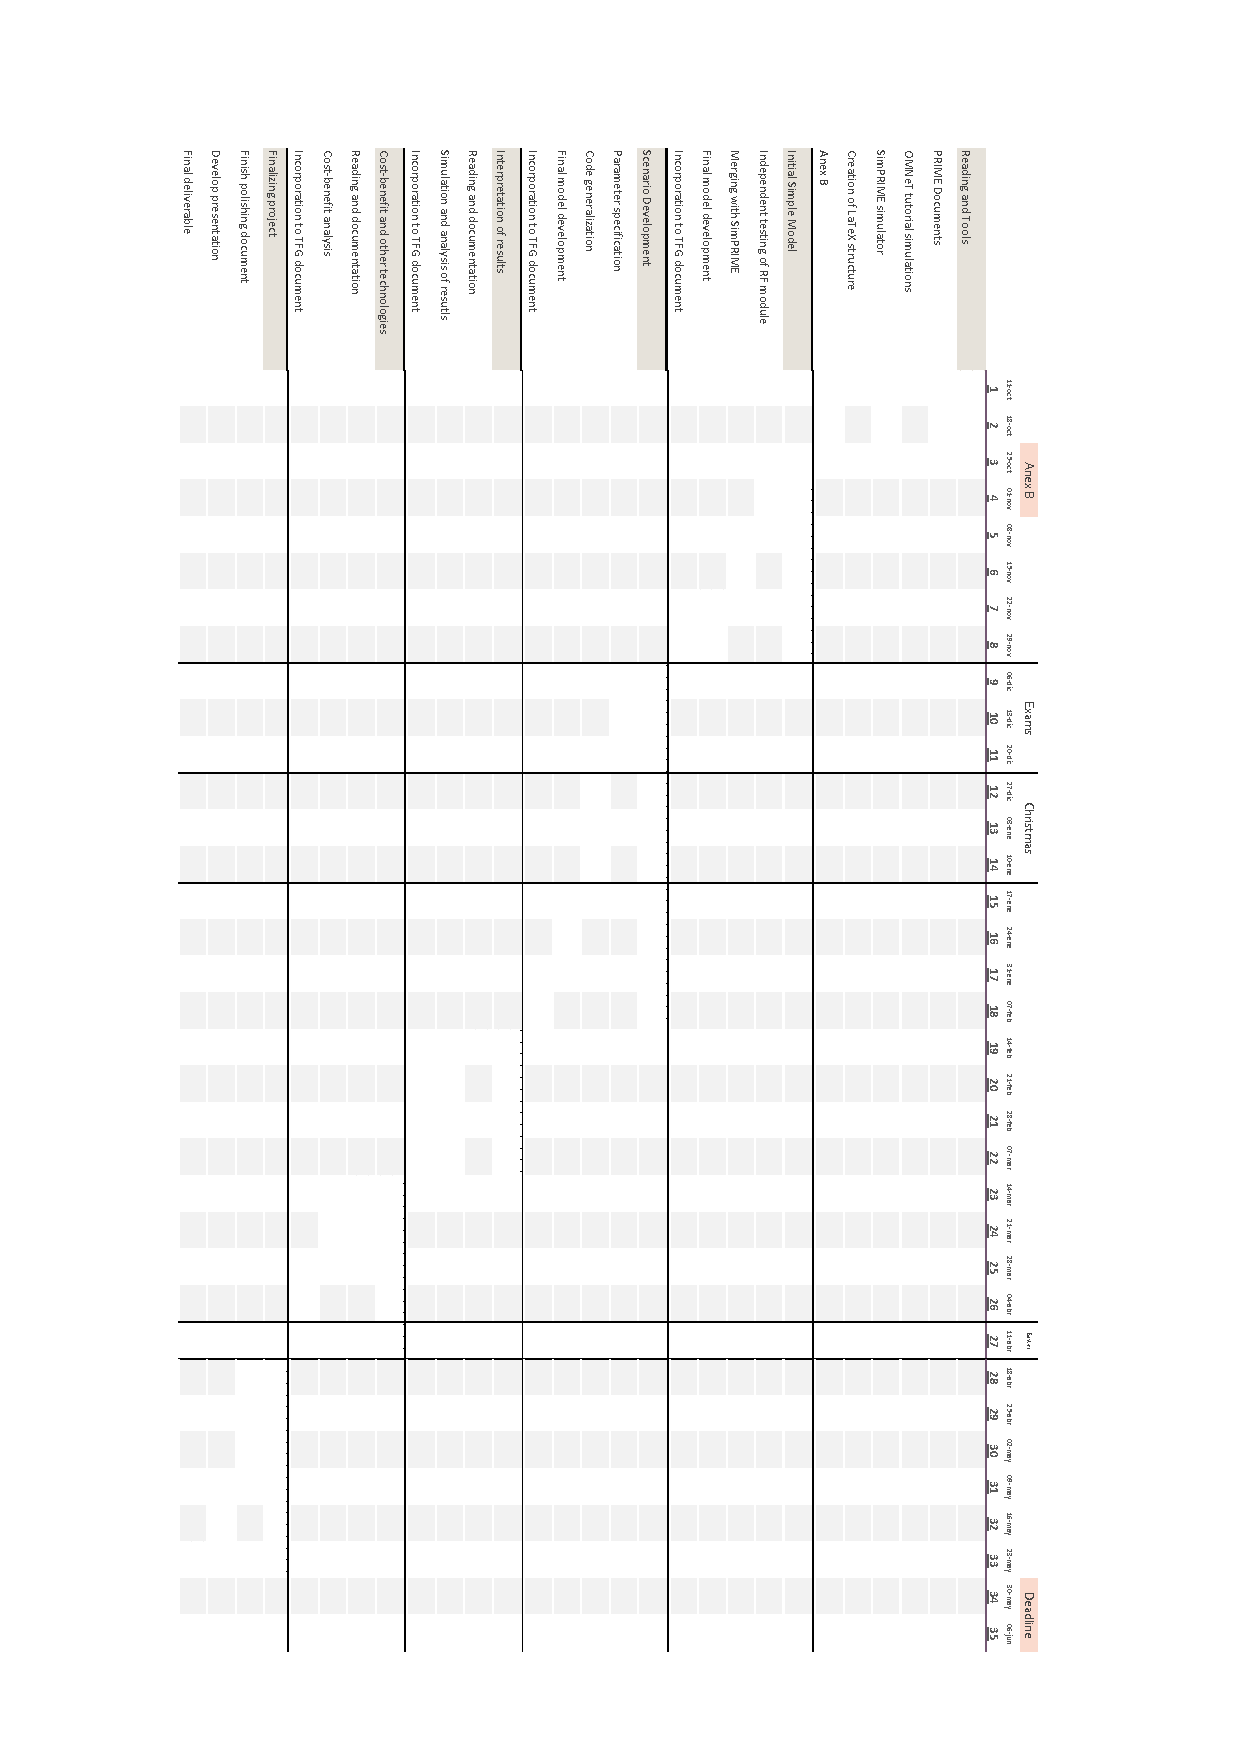
\includepdf[pages=-]{images/planning.pdf}
	
\end{document}
